% Manifest-bound publication figure includes. Vector PDF is the publication path.

\begin{figure*}[t]
  \centering
  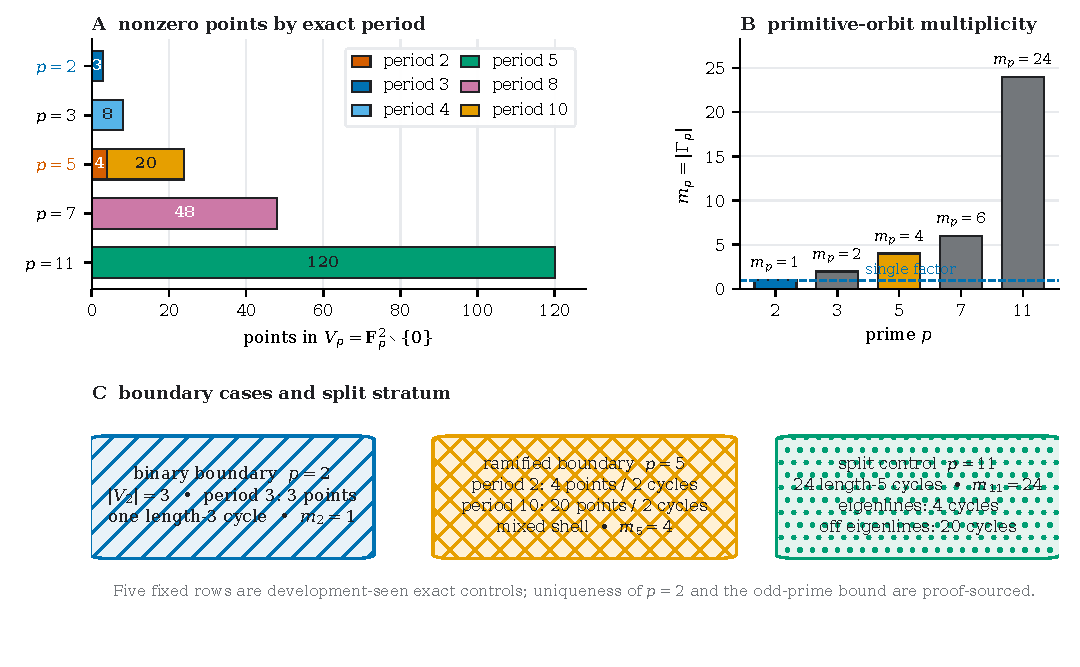
\includegraphics[width=\textwidth]{figures/fig1_shell_profiles.pdf}
  \caption{%
    Exact profiles on the five frozen prime shells.  (A) Nonzero points are
    partitioned by least return period.  (B) The resulting primitive-orbit
    multiplicity is (m_p=1,2,4,6,24) for
    (p=2,3,5,7,11), respectively.  (C) The binary shell is the sole
    one-orbit boundary, the ramified (p=5) shell mixes two length-two with
    two length-ten cycles, and the split (p=11) control separates four
    eigenline from twenty off-eigenline cycles.  These fixed rows are
    development-seen exact controls; uniqueness of (p=2) and the all-odd
    lower bound are proof-sourced, not inferred from the finite display.}
  \label{fig:prime-shell-profiles}
\end{figure*}

\begin{figure*}[t]
  \centering
  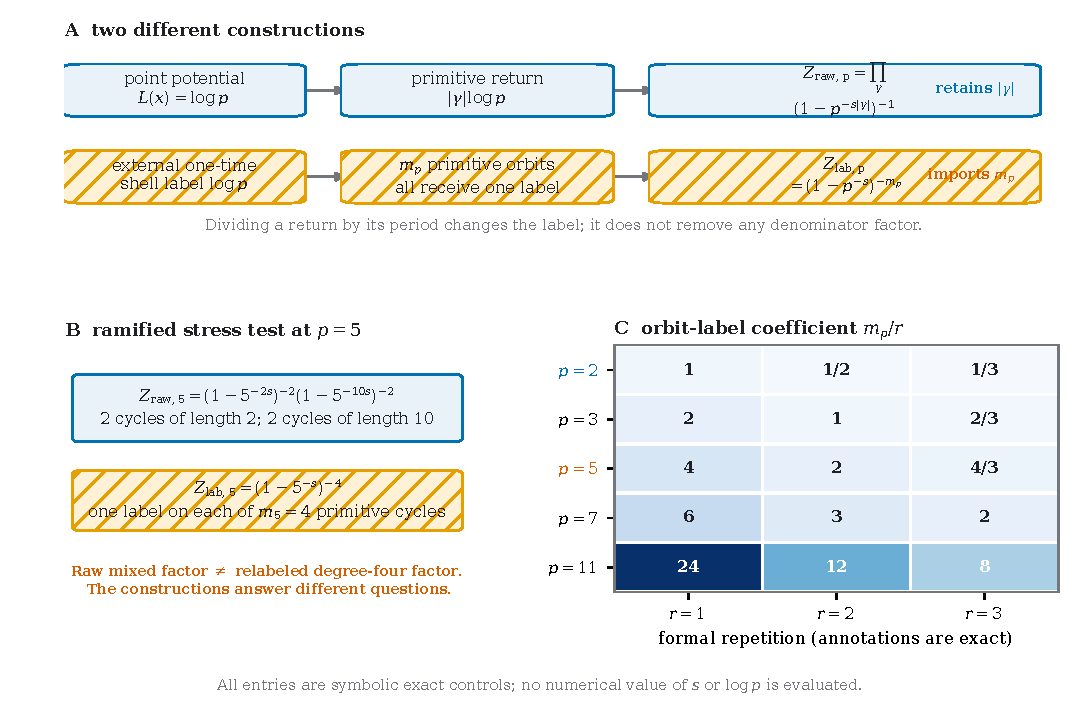
\includegraphics[width=\textwidth]{figures/fig2_product_semantics.pdf}
  \caption{%
    The point-potential return product and the externally relabeled orbit
    product are different constructions.  (A) A genuine return retains the
    primitive length (|\gamma|), whereas assigning (log p) once per
    primitive orbit imports the multiplicity (m_p).  (B) At the ramified
    prime, the raw factor has separate length-two and length-ten monomials,
    while the label factor has degree four in the one-time shell label.
    (C) The exact formal repetition coefficient is (m_p/r) for
    (r=1,2,3).  No numerical value of (s) or (log p) is evaluated.}
  \label{fig:raw-versus-label}
\end{figure*}

\begin{figure*}[t]
  \centering
  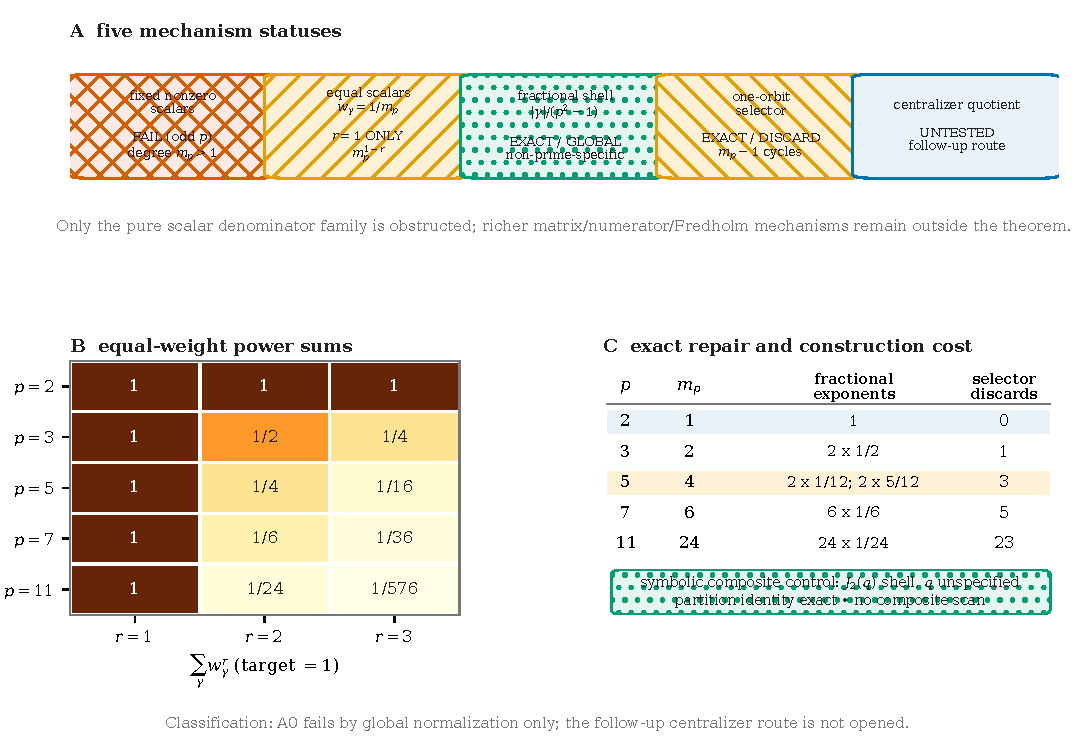
\includegraphics[width=\textwidth]{figures/fig3_mechanism_boundary.pdf}
  \caption{%
    Mechanism boundary for collapsing shell multiplicity.  (A) Fixed
    nonzero scalar denominators fail by degree on every odd shell; equal
    weights repair only the first repetition; fractional exponents give an
    exact but shell-global identity; a one-orbit selector succeeds only by
    discarding (m_p-1) cycles; and a centralizer quotient remains an
    untested follow-up route.  (B) Exact equal-weight power sums at the three
    frozen repetitions.  (C) Fractional outer exponents sum to one and the
    selector costs are exact.  The symbolic (J_2(q)) control shows that the
    fractional partition identity is not prime-specific; no composite shell
    was enumerated.}
  \label{fig:mechanism-boundary}
\end{figure*}
